\documentclass[11pt,a4paper,onesides]{report}
\usepackage{graphicx}
\DeclareGraphicsExtensions{.pdf,.png,.jpg}



\begin{document}


\title{User Interface and Embedded System  \\ Technical Report}
\author{Paul Glotfelter}
\date{August 2014}
\maketitle

\chapter{Introduction}

This report covers the research, design, analysis, and prototyping of the team 2 Automated Bike Rental Station (ABRS).  In particular, the report discusses the initial requirements and expectations, the research to investigate the initial criteria, the analysis of the proposed model, and the prototyping of the proposal involving the embedded system and user interface of the project.  

\chapter{Initial Requirements}

The initial requirements were set forth in the form of a system from which customers can rent bicycles.  The purpose of this product is to enrich the communication and relationship between York College and its surrounding community.  To facilitate this project, certain major specifications are required from the ABRS system.  The bike rack must be able to operate year-round, customers return bikes to the same stations from which they were rented, and the ABRS must be able to sufficiently power itself when a grid connection is unavailable.  These criteria present unique problems to each engineering group working on the project.  However, this report specifically covers the requirements the criteria imposed on the computer engineering portion of the ABRS.  

\section{General Guidelines}

The general guidelines are: the ABRS must consist of a kiosk (a central unit housing the display and handling customer interactions) and one to five bike modules.  Each bike module will house five bikes with individual locking stations for each one.  The entire unit must be generally resilient to physical damage.  In addition, it must be completely safe for operation with young children as well as adults.    

\section{Operating Conditions}

In order for the bike system to operate year round, the components selected for the rack must be able to withstand the extreme temperature variations of the hot and cold weather experienced in the York, Pennsylvania area.  The ABRS must also be intuitive and simple to use in each of these weather conditions.  Additionally, the ABRS may be located in city areas.  So, its components should be highly resistant to vandalism and theft. 

\section{Return Procedure}

As this is a product being designed for the general consumer, the end result is to be as intuitive and simple as possible.  Thus, when customers return bicycles, the checkout procedure must be straightforward.  Under optimal conditions, the customers will simply return the bicycle to the ABRS and their account will be appropriately charged.  In order for the system to discern which bike is being returned, it must be able to uniquely identify bikes.

\section{System Power}

 The ABRS system aims to be totally self-sufficient in terms of supplying power to the components.  However, it must also be able to connect to the grid when necessary.  Therefore, the components must be selected with these goals in mind.  That is, the power consumption of the components must be low so that the system can be self-sufficient.  In addition, power-saving protocols for the UI may also be required.  

\chapter{Initial Developments}

\section{Communications Protocol}

In general, the system can be described as a central kiosk unit communicating by some protocol to each of the individual bike modules.  This description is the core of the ABRS from an engineering perspective.  Thus, the initial research and development began with communication strategies.  

The initial thought was to use wireless communication for this purpose.  Wireless communication ubiquitous in modern systems.  In addition, it allows for easy communication between the kiosk and each bike module.  However, it does present an entirely new set of problems to address: the wireless communications must be encrypted and each bike module must be equipped with an embedded component capable of handling wireless transmission, adding additional cost to the system.  

Because of the issues with wireless communication,  it is far more efficient in terms of time and cost to use a wired approach.  In particular, a scheme in which the kiosk is directly connected to each of the bike modules and directly controls the bike locking mechanisms (discussed further in section ???), resulting in the rough system model shown in Figure-1.  

%0.6 seems to be a really good size for figures :)

\begin{figure}[h]
	\begin{center}
		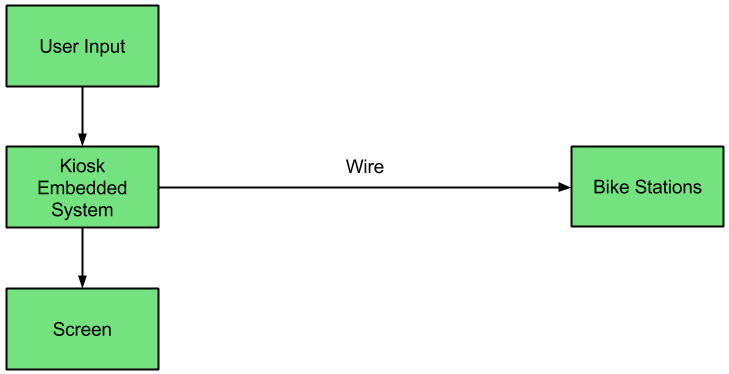
\includegraphics[scale = 0.6]{initial-diagram}
	\end{center}
\caption{Figure-1:  A preliminary diagram of the system}

\end{figure}

\section{User Interactions}

The chosen display for the ABRS is an industrial LCD screen.  The manner in which the system interacts with the user is the single most important goal for the ABRS to achieve.  The system must offer an interface that is aesthetically pleasing and intuitive to navigate.  These criteria guided the team to initially discuss using a touchscreen for the kiosk display.  However, background research revealed that the temperature ranges in York, Pennsylvania would be too harsh for a touchscreen to operate effectively in all conditions.  In addition, touchscreens would be highly uncomfortable to use in winter weather.  An LCD would allow for intuitive usage as well as temperature resistivity and physical endurance.



\end{document}